%20 min preso!
\documentclass[aspectratio=169,xcolor=table,english]{beamer}
\usepackage{beamerthemesplit}
\usepackage{wrapfig}
\usetheme{SPbGU}
\usepackage{pdfpages}
\usepackage{amsmath}
\usepackage{mathtools}
\usepackage{cmap}
\usepackage{subcaption}
\usepackage[utf8]{inputenc}
\usepackage[T1, T2A]{fontenc}
\usepackage[]{babel}
\usepackage{indentfirst}
\usepackage{amsmath}
\usepackage{tikz}
\usepackage{multirow}
\usepackage[noend]{algpseudocode}
\usepackage{algorithm}
\usepackage{algorithmicx}
\usepackage{fancyvrb}
\usetikzlibrary{calc}
\usetikzlibrary{shapes,arrows}
\usetikzlibrary{arrows,automata}
\usetikzlibrary{positioning}
\usetikzlibrary{fit}

\usepackage{kbordermatrix} % include package @ document preamble
\renewcommand{\kbldelim}{(} % change default array delimiters to parentheses
\renewcommand{\kbrdelim}{)}

\newcommand\mca{\multicolumn{1}{c}{\cellcolor{red}\textbf{\{a\}}}}
\newcommand\mcb{\multicolumn{1}{c}{\cellcolor{red}\textbf{\{b\}}}}

\usepackage{tabularx}
\newcolumntype{Y}{>{\raggedleft\arraybackslash}X}

\renewcommand{\thealgorithm}{}

\newtheorem{mytheorem}{Theorem}
\renewcommand{\thealgorithm}{}

\newcommand{\tikzmark}[1]{\tikz[overlay,remember picture] \node (#1) {};}
\def\Put(#1,#2)#3{\leavevmode\makebox(0,0){\put(#1,#2){#3}}}

\newcommand{\ltz}{$< 1$}

\tikzset{
    state/.style={
           rectangle,
           rounded corners,
           draw=black, very thick,
           minimum height=2em,
           inner sep=2pt,
           text centered,
           },
}

\beamertemplatenavigationsymbolsempty

\title[SPLA]{Generalized sparse linear algebra framework for multi-GPU computations}
% \subtitle[YaccConstructor]{Parsing techniques for graph analysis}
% То, что в квадратных скобках, отображается в левом нижнем углу.
\institute[SPbU]{
Scientific supervisor: C.Sc., docent S.V. Grigorev\\
Saint Petersburg State University
}

% То, что в квадратных скобках, отображается в левом нижнем углу (прикольно).
\author[Egor Orachev]{\textbf{Egor Orachev, 21.М07-мм}}
\date{December 29, 2021}


\begin{document}
{
\begin{frame}[fragile]
  \begin{table}
  \centering
  \begin{tabularx}{\linewidth}{YcX}
        \begin{minipage}[t]{\textwidth}\center \vspace{0.2cm}             
\includegraphics[height=2.0cm]{pictures/SPbGU_Logo.png} 
        \end{minipage}
     \hfill 
  \end{tabularx}
  \end{table}
  \titlepage
\end{frame}
}

\begin{frame}[fragile] \frametitle{Introduction}
    \begin{minipage}[m]{0.5\linewidth}
        \textbf{Sparse linear algebra framework}:
        \begin{itemize}
            \item Practical problem solving
            \item High-perforce libraries
            \item Values' types and functions
            \item Primitives: matrix, vector, scalar
            \item Operations: mxm, vxm, mxv, assign, reduce, transpose
        \end{itemize}
        \vspace{0.2cm}
        \textcolor{red}{Note 1: practical data are sparse\\Note 2: practical data are large}
    \end{minipage}\hfill
    \begin{minipage}[m]{0.45\linewidth}
        \begin{figure}
            \centering
            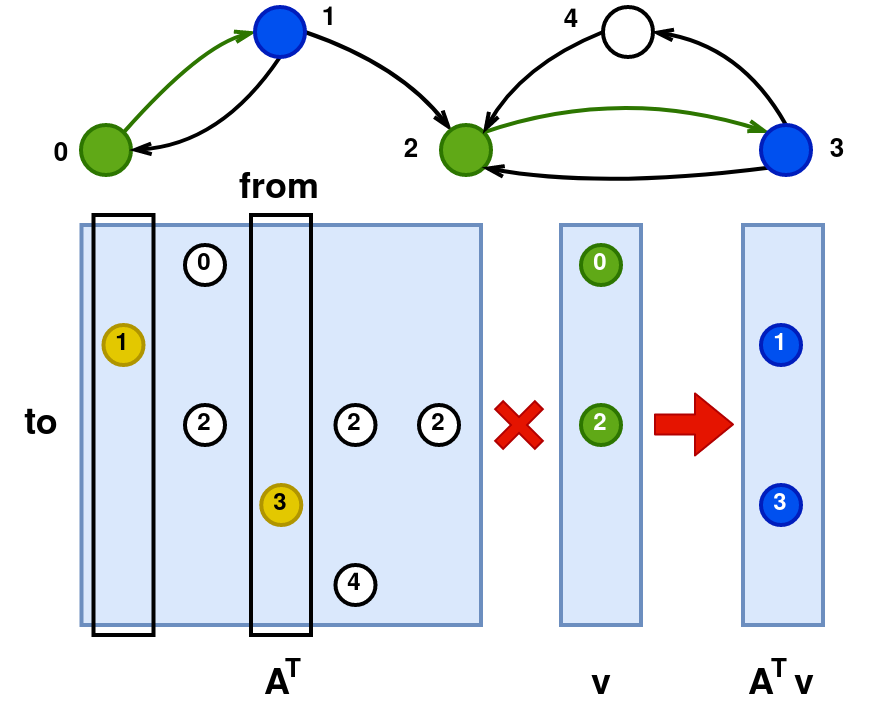
\includegraphics[width=\textwidth]{figures/graph_traversal.png}
            \caption{Graph traversal by matrix-vector multiplication}
            \label{fig:traversal}
        \end{figure}
    \end{minipage}
\end{frame}

\begin{frame}[fragile] \frametitle{Applications}
    \begin{minipage}[m]{0.5\linewidth}
        \begin{itemize}
            \item \textbf{Algorithms}
            {
            \begin{itemize}
                \item Breadth-first search
                \item Shortest paths
                \item Maximal independent set
                \item Page rank
                \item Triangles counting 
                \item Regular/CFL-reachability
            \end{itemize}
            }
            \item \textbf{Analysis tasks}
            {
            \begin{itemize}
                \item Static code analysis
                \item Graph database queries
                \item Bioinformatics
            \end{itemize}
            }
        \end{itemize}
    \end{minipage}\hfill
    \begin{minipage}[m]{0.5\linewidth}
        \begin{figure}
            \centering
            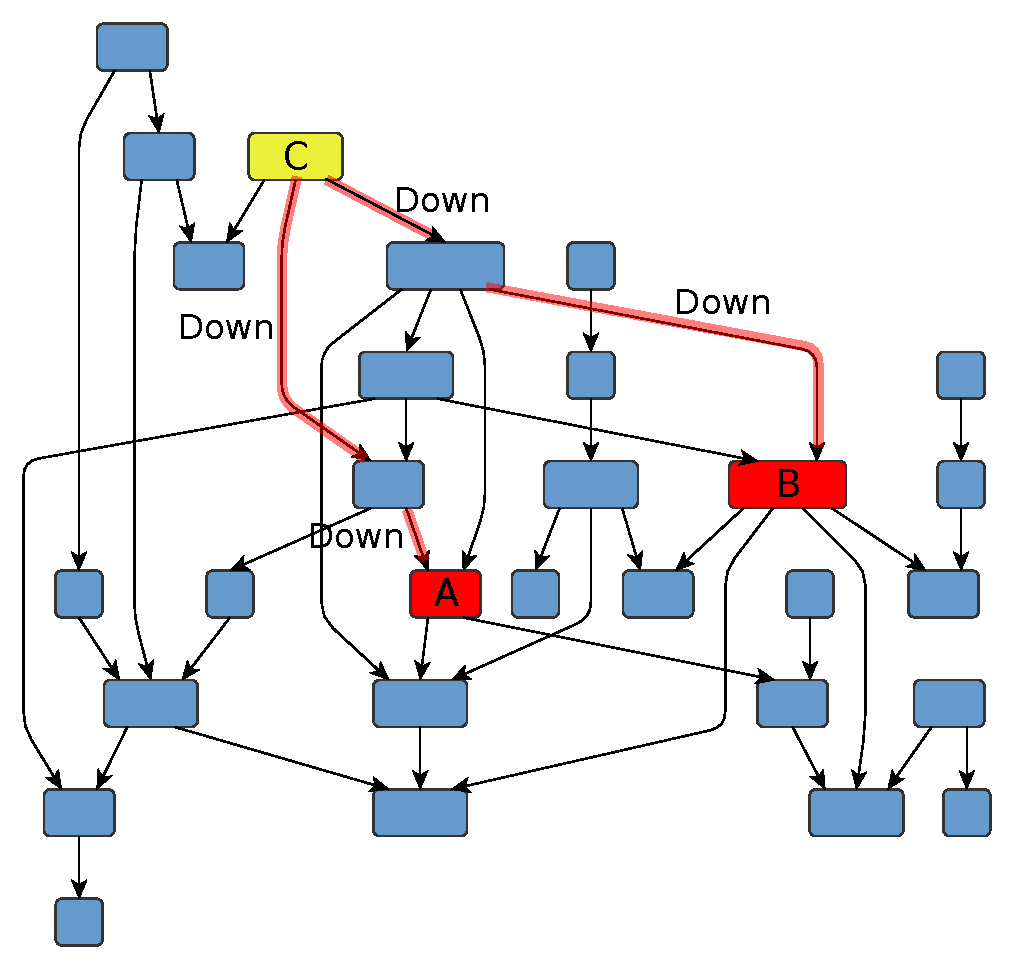
\includegraphics[width=0.8\textwidth]{pictures/hierarchical.pdf}
            \caption{Navigational query $\overline{\textbf{Down}}^n$$\textbf{Down}^n$ for CFL-reachability}
            \label{fig:navigation}
        \end{figure}
    \end{minipage}
\end{frame}

\begin{frame}[fragile] \frametitle{Background}
    \begin{minipage}[m]{0.7\linewidth}
        \begin{itemize}
        \item GraphBLAS
        {
        \begin{itemize}
            \item Mathematical notation translated into an C API
        \end{itemize}
        }
        \item GraphBLAS:SuiteSparse
        {
        \begin{itemize}
            \item GraphBLAS reference implementation
            \item CPU-computations \& high-performance
        \end{itemize}
        }
        \item GraphBLAST
        {
        \begin{itemize}
            \item CUDA C++ template based
            \item Under-development | abandoned
        \end{itemize}
        }
        \item cuSPARSE, clSPARSE, bhSPARSE, GALATIC, cusp
        {
        \begin{itemize}
            \item General-purpose sparse linear algebra libraries
            \item Under-development | outdated | single-GPU
        \end{itemize}
        }
        \item SPbLA, cuBool
        {
        \begin{itemize}
            \item OpenCL | CUDA | CPU
            \item Single-GPU \& optimized \& boolean values only
        \end{itemize}
        }
        \end{itemize}
    \end{minipage}\hfill
    \begin{minipage}[m]{0.3\linewidth}
        \begin{figure}
            \centering
            
\includegraphics[width=\textwidth]{figures/graphblas-logo.png}
            \caption{GraphBLAS project logo (picture from graphblas.org)}
            \label{fig:graphmlas}
        \end{figure}
    \end{minipage}
\end{frame}

\begin{frame}[fragile] \frametitle{Project: motivation and tasks}
    \begin{minipage}[m]{0.7\linewidth}
        \begin{itemize}
            \item \textbf{Motivation}
            {
            \begin{itemize}
                \item No complete and ready for usage\\GPU GraphBLAS implementation
                \item Existing math libraries limited in customization
                \item No multi-GPU support
            \end{itemize}
            }
            \item \textbf{Idea}
            {
            \begin{itemize}
                \item Generalized sparse linear algebra framework
                \item Verbose and declarative API
                \item No templates $\Rightarrow$ C and Python wrapping
            \end{itemize}
            }
            \item \textbf{Challenges}
            {
            \begin{itemize}
                \item GPU programming is hard!
                \item Compute APIs verbose and low-level
                \item Numerous algorithms for particular operations
            \end{itemize}
            }
        \end{itemize}
    \end{minipage}\hfill
    \begin{minipage}[m]{0.3\linewidth}
        \begin{figure}
            \centering
            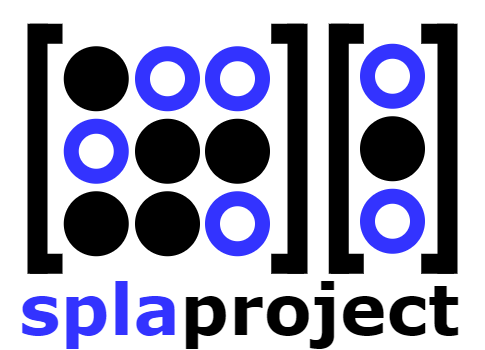
\includegraphics[width=\textwidth]{figures/spla-logo.png}
            \caption{SPLA project logo (picture from spla project page)}
            \label{fig:logo}
        \end{figure}
    \end{minipage}\hfill
\end{frame}

\begin{frame}[fragile] \frametitle{Requirements}
    \begin{minipage}[m]{0.55\linewidth}
        \begin{itemize}
            \item User-defined types support
            \item User-defined functions support 
            \item DAG-based expressions
            \item Automated internal hybrid storage format
            \item Automated multi-GPU work scheduling
        \end{itemize}
    \end{minipage}\hfill
    \begin{minipage}[m]{0.45\linewidth}
        \begin{figure}
            \centering
            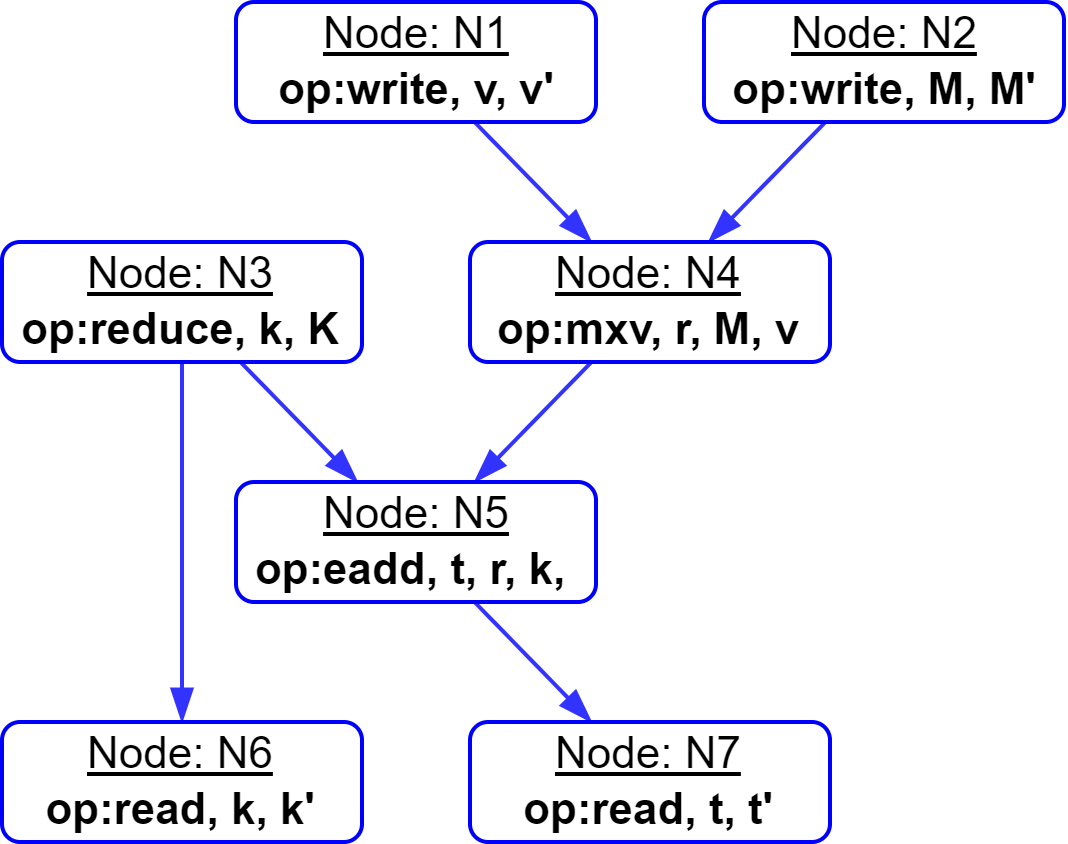
\includegraphics[width=0.85\textwidth]{figures/example_expression.png}
            \caption{Example computational expression in DAG form. Note dependencies between nodes.}
            \label{fig:example_expression}
        \end{figure}
    \end{minipage}
\end{frame}

\begin{frame}[fragile] \frametitle{Implementation details}
    \begin{minipage}[m]{0.55\linewidth}
        \begin{itemize}
            \item \textbf{Dev-stack}: 
            { 
            \begin{itemize}
                \item C++17, CMake, C 99, Python 3
                \item Compute API: OpenCL 1.2\footnotemark[1]
                \item Aux compute library: boost.compute\footnotemark[2]
                \item Tasking library: taskflow\footnotemark[3]
            \end{itemize} 
            }
            \item \textbf{Strategy}: 
            {
            \begin{itemize}
                \item Write generalized cl kernels
                \item Utilize boost meta-kernels library
                \item Handle values as raw byte sequences (POD)
                \item User-defined functions effectively are strings
            \end{itemize}
            }
        \end{itemize}
    \end{minipage}\hfill
    \begin{minipage}[m]{0.45\linewidth}
        \begin{figure}
            \centering
            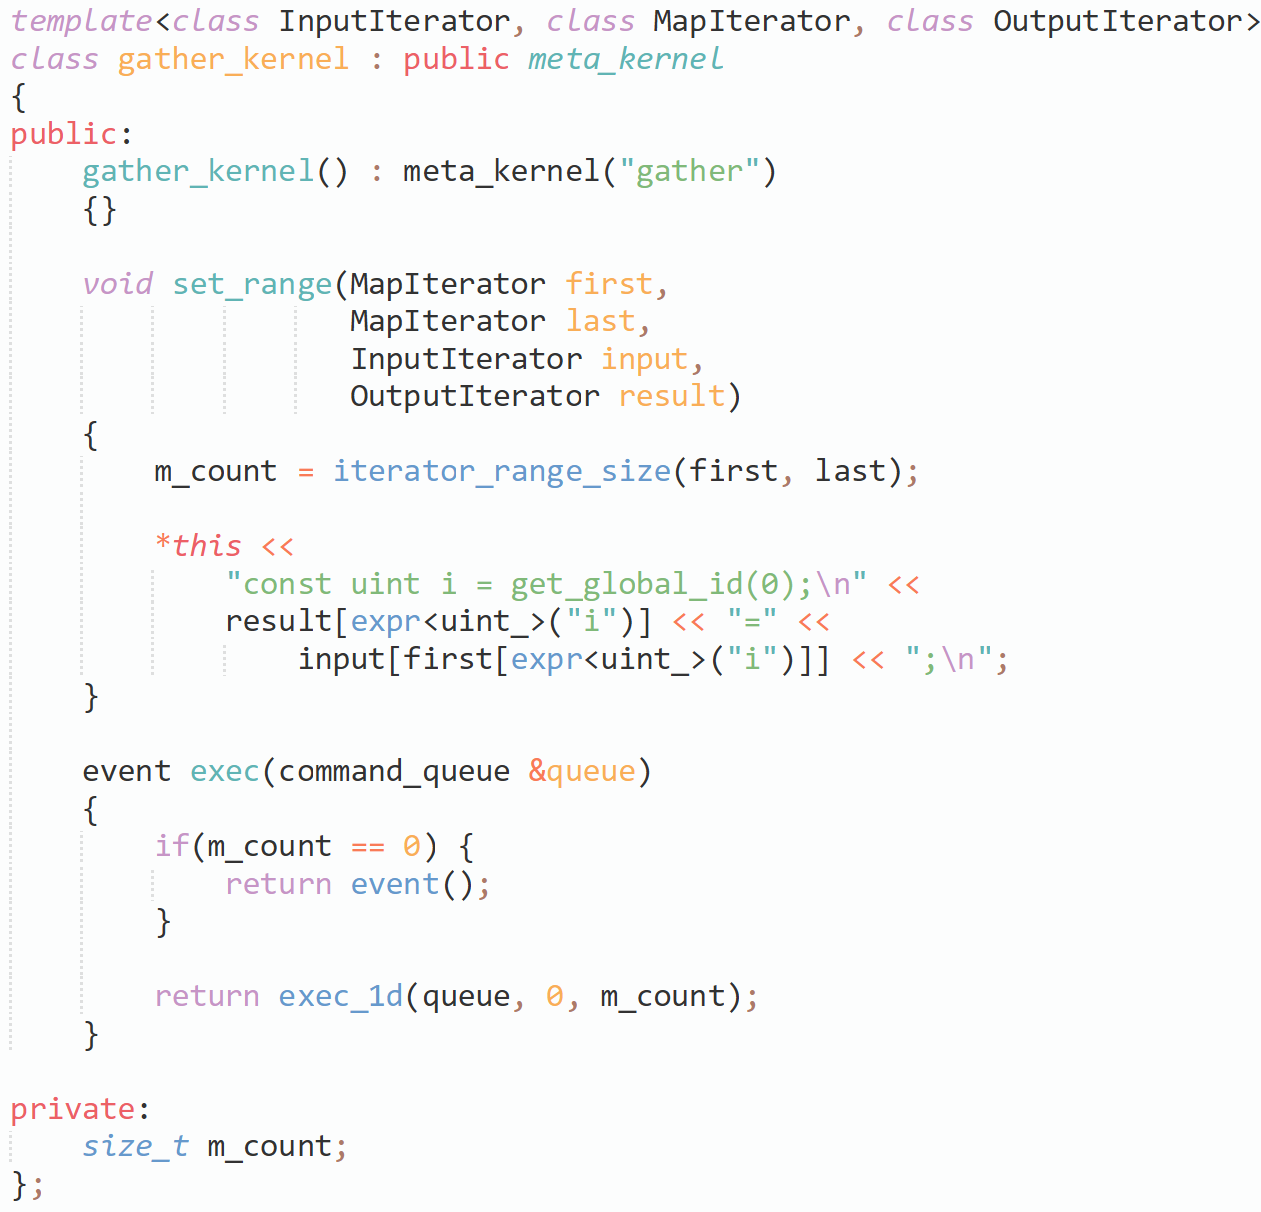
\includegraphics[width=0.75\textwidth]{figures/meta_programming.png}
            \caption{Gather OpenCL meta-kernel (picture from boost.compute library)}
            \label{fig:meta_programming}
        \end{figure}
    \end{minipage}
    
    \footnotetext[1]{\href{https://www.khronos.org/opencl/}{https://www.khronos.org/opencl/}}
    \footnotetext[2]{\href{https://github.com/boostorg/compute}{https://github.com/boostorg/compute}}
    \footnotetext[3]{\href{https://github.com/taskflow/taskflow\#dynamic-tasking}{https://github.com/taskflow/taskflow\#dynamic-tasking}}
\end{frame}

\begin{frame}[fragile] \frametitle{Issues}
    \begin{minipage}[m]{0.55\linewidth}
        \begin{itemize}
            \item Work distribution between computational units
            \item Host-device synchronization
            \item Computational dependencies
            \item Storage format and data sharing
            \item Efficient CPU usage
        \end{itemize}
    \end{minipage}\hfill
    \begin{minipage}[m]{0.45\linewidth}
        \begin{figure}
            \centering
            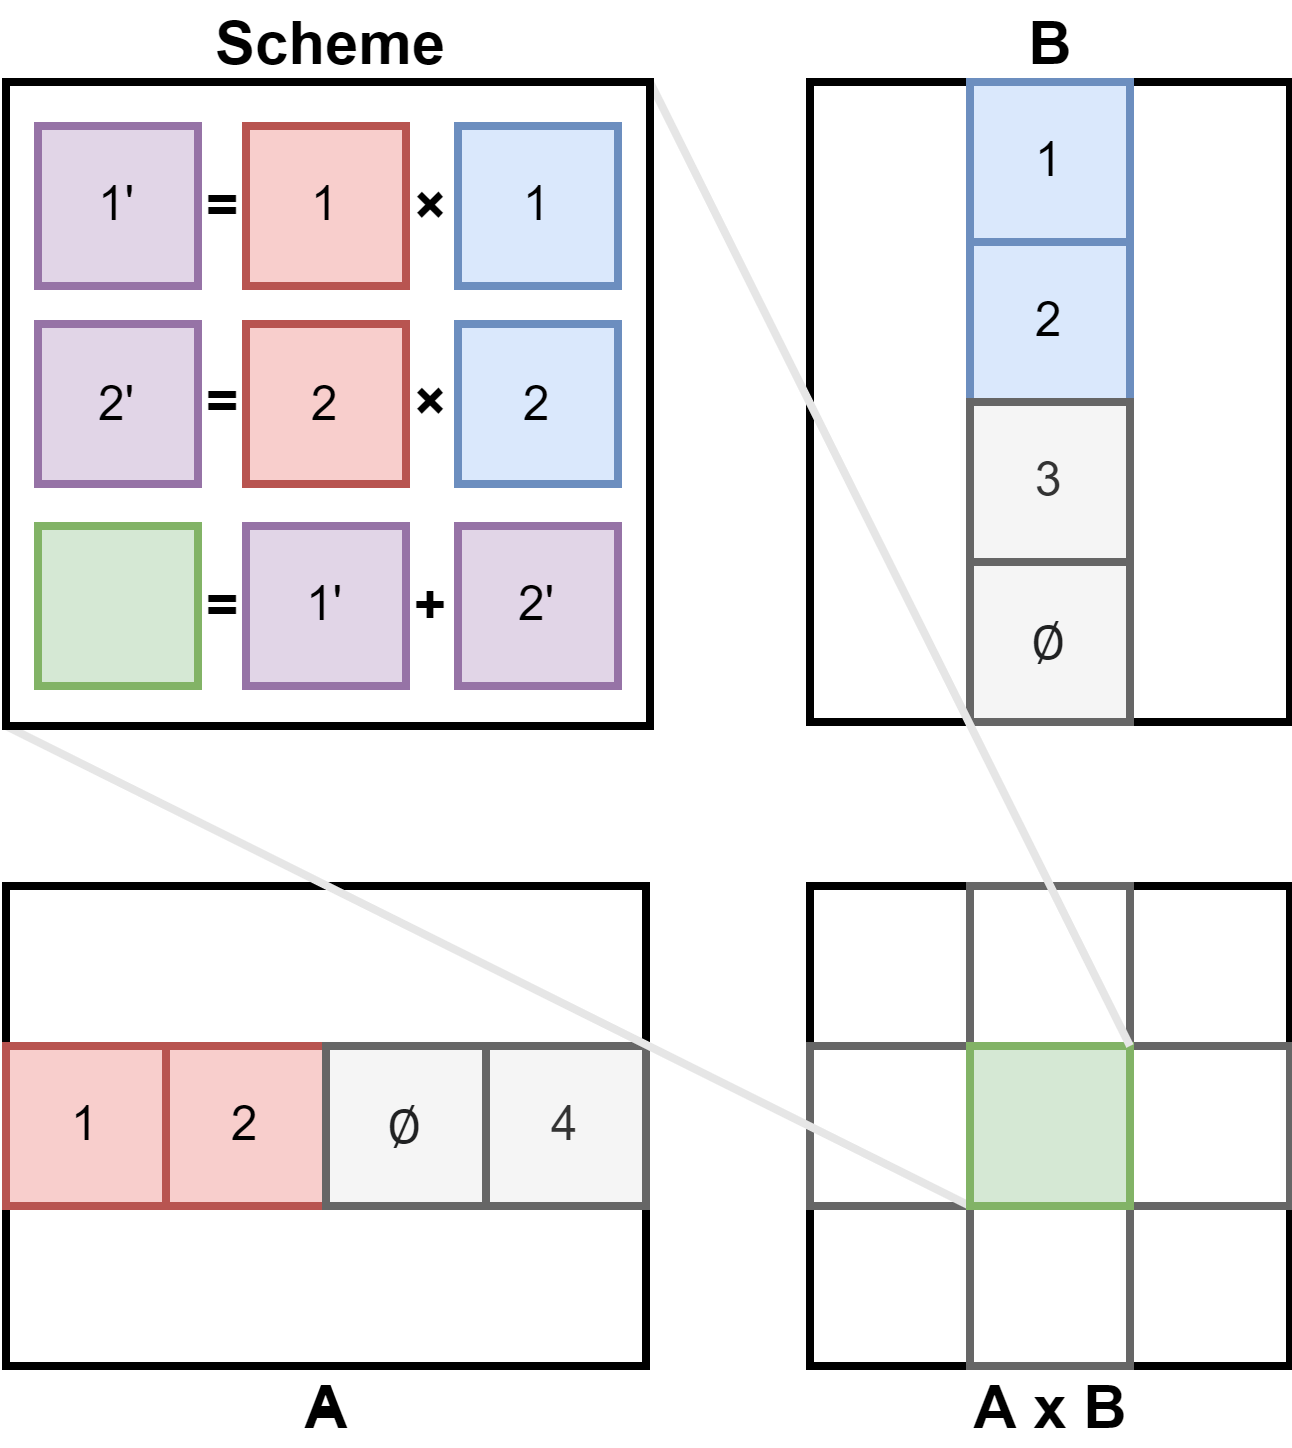
\includegraphics[width=0.6\textwidth]{figures/blocked_storage.png}
            \caption{Example blocked sparse matrix storage. Evaluation of $A \times B$ for some result block. Note, each temporary block product is fully independent GPU task.}
            \label{fig:blocked_storage}
        \end{figure}
    \end{minipage}
\end{frame}

\begin{frame}[fragile] \frametitle{API Usage example}
    \begin{center}
    \begin{minipage}[m]{0.9\linewidth}
        \begin{figure}
            \centering
            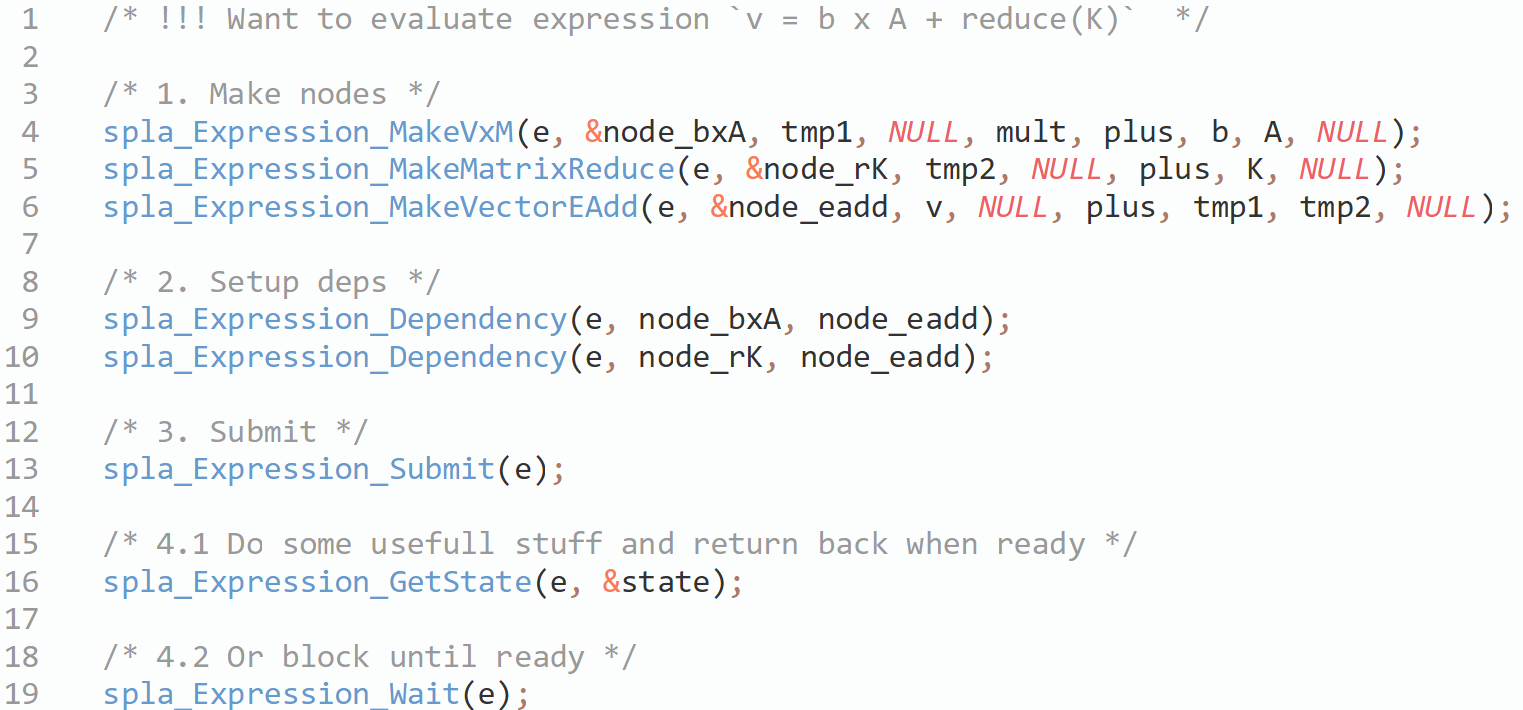
\includegraphics[width=0.8\textwidth]{figures/c_api_expression.png}
            \caption{Evaluation of $v = b \times A + \textit{reduce}(K)$ using \textbf{spla C API}, where $v$, $b$ are vectors, $A$ and $K$ are matrices, defined somewhere earlier in the code. DAG is set up using expression node dependencies. Note, that we use generic \textit{plus} and \textit{mult}, which can be defined by the user.}
        \end{figure}
    \end{minipage}\hfill   
    \end{center}
\end{frame}

\begin{frame}[fragile] \frametitle{Progress}
    \begin{itemize}
        \item C++ Core API
        \item Primitives: matrix, vector, scalar
        \item Operations: mxm, vxm, assign, eadd
        \item Algorithms: \textit{bfs}, \textit{sssp}
        \item Hybrid storage format
        {
        \begin{itemize}
            \item Generic blocked matrix, vector
            \item COO-format blocks 
            \item Empty blocks not stored
            \item It is possible to add CSR, DCSR, Dense blocks
        \end{itemize}
        }
        \item Task-graph
        {
        \begin{itemize}
            \item Task for each DAG's node
            \item Separate set of sub-tasks inside each node's task
            \item Each sub-task is assigned to concrete GPU
        \end{itemize}
        }
    \end{itemize}
\end{frame}

\begin{frame}[fragile] \frametitle{Roadmap}
    \begin{itemize}
        \item Operations: reduce, emult, transpose
        \item Algorithms: \textit{tc}, \textit{page-rank}, \textit{connected-components}, etc.
        % \item GrAPL 2022 workshop\footnote{\href{https://hpc.pnl.gov/grapl/}{https://hpc.pnl.gov/grapl/}}
        % \item Joss journal paper\footnote{\href{https://joss.theoj.org/}{https://joss.theoj.org/}}
        % \item Graphalytics competitions\footnote{\href{https://ldbcouncil.org/benchmarks/graphalytics/}{https://ldbcouncil.org/benchmarks/graphalytics/}}
        \item Fine tuning: optimizations, state of the art SpGEMM's
        \item C API wrapper \& Python package (PyPI publication)
    \end{itemize}
\end{frame}

\begin{frame} \frametitle{Also}
    \begin{itemize}
        \item SPLA project: \href{https://github.com/JetBrains-Research/cuBool}{https://github.com/JetBrains-Research/spla}
        \item Email: \href{mailto:egororachyov@gmail.com}{egororachyov@gmail.com}
        \item Materials:
        {
            \begin{itemize}
                \item Szuppe, J. 2016. Boost.Compute: A parallel computing library for C++ based on OpenCL. Proceedings of the 4th International Workshop on OpenCL.
                \item Timothy A. Davis. 2019. Algorithm 1000: SuiteSparse:GraphBLAS: Graph Algorithms in the Language of Sparse Linear Algebra. ACM Trans. Math. Softw. 45, 4, Article 44 (December 2019), 25 pages. DOI:https://doi.org/10.1145/3322125
                \item E. Orachev, M. Karpenko, A. Khoroshev and S. Grigorev. 2021. "SPbLA: The Library of GPGPU-Powered Sparse Boolean Linear Algebra Operations," IEEE International Parallel and Distributed Processing Symposium Workshops (IPDPSW), 2021, pp. 272-275, doi: 10.1109/IPDPSW52791.2021.00049.
            \end{itemize}
        }
    \end{itemize}
\end{frame}

\end{document}
